\chapter{Functional}

Functional refers to a mapping of functions or curves (belonging to a certain set) to a definite number. Details are introduced in this chapter.

\section{A Motivating Example}

One of the most famous problems solved by functional and calculus of variation is the brachistochrone problem, which is described in the box below.

\begin{shortbox}
\Boxhead{Brachistochrone Problem}

Let A and B be two fixed points in a vertical plane, where A is higher than B (from gravity perspective) and A, B are not aligned vertically. Draw a curve that joins A and B. A particle is released from A and it slides along the curve traveling from A to B driven by gravity. The velocity of the particle, at any given position, is decided by the position of the particle relevant to $A$ (speed) and the tangent of the curve at the particle position (direction). A demonstration is given by Fig. \ref{ch12fig:brachistochrone_description}.

The brachistochrone problem tries to find the curve that minimizes the time it takes for the particle to travel from A to B. The objective is to find the analytical solution $y=f(x)$ that describes such curve.

\end{shortbox}

\begin{figure}
	\centering
	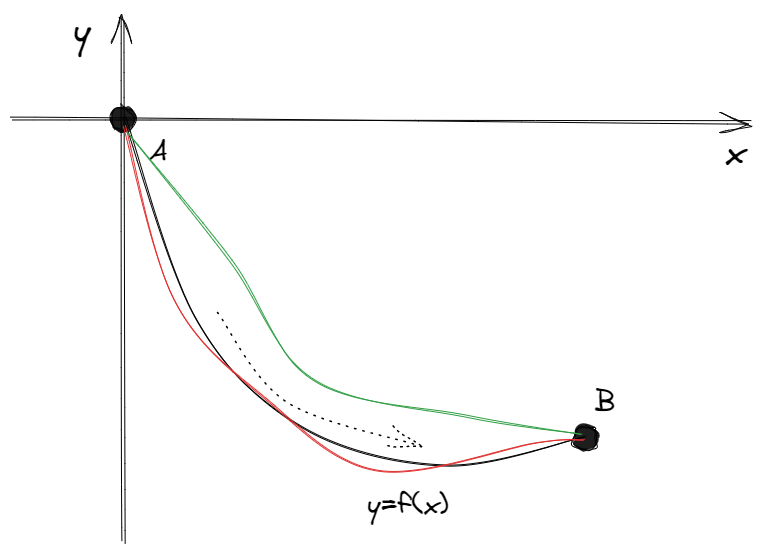
\includegraphics[width=200pt]{chapters/part-4/figures/brachistochrone_description.png}
	\caption{Brachistochrone problem description.} \label{ch12fig:brachistochrone_description}
\end{figure}

\section{Functional}

Definition of functional as well as its relationship with the associated finite differences approximation is explained as follows.

\subsection{Definition}

Functional can be regarded as an extension to function, where the input is not a variable or a set of variables, but a function. Functional has many practical applications in data analysis, mechanics, geometry, control systems, etc. Many optimization problems are also defined using functional.

Let $y(x)$ be a function of $x$. Let $J[y]$ be a functional of $x$, $y$ and values derived from them. For example, $J[y]$ may look like
\begin{eqnarray}
	J = \int_{a}^{b} \sqrt{1+y\prime^2} dx \nonumber
\end{eqnarray}
which is the length of curve $y(x)$ from $x=a$ to $x=b$. The study of $J[y]$ with different choice of $y(x)$ is called ``calculus of functional''. 

Calculus of functional is often difficult to solve. Calculus of variation is a special case of calculus of functional that only studies the choice of $y$ that maximizes or minimizes $J$. Even with that been said, calculus of variation is still difficult to solve in general, and the analytical solution of $y(x)$ exists for only certain forms of $J$. This notebook only considers a small subset of the problem where $J$ follows the following form
\begin{eqnarray}
	y &=& y(x) \nonumber \\
	J &=& \int_{a}^{b}F\left(x, y, y\prime \right)dx \label{eq:covbasiceq}
\end{eqnarray}
Notice that the above functional \eqref{eq:covbasiceq} has a ``localization property'', where if the curve $y(x)$ is split into segments whose functional calculated separately, the sum of the values of the functional would be equal to the functional of the whole curve. This does not generally apply if $J$ is defined arbitrarily with a different form as given by \eqref{eq:covbasiceq}. For example, consider
\begin{eqnarray}
	J &=& \frac{\int_{a}^{b}x\sqrt{1+y\prime^2}dx}{\int_{a}^{b}\sqrt{1+y\prime^2}dx} \nonumber
\end{eqnarray}
which does not follow \eqref{eq:covbasiceq} and it is a non-local functional.

\subsection{Finite Differences Approximation}

An intuitive way of solving the calculus of variation is as follows. Let $x_i$, $i=0,...,n+1$ be samples uniformly taken from $[a,b]$ where $x_0 = a$ and $x_{n+1}=b$, and $y_i = y(x_i)$. With localization property, \eqref{eq:covbasiceq} can be approximated by the following finite differences
\begin{eqnarray}
	J[y] &\approx&  \sum_{i=1}^{n+1} F\left(x_i, y_i, \frac{y_i-y_{i-1}}{h}\right) \label{eq:covapprox}
\end{eqnarray}
where $h=x_{i+1}-x_i$. When $n\rightarrow\infty$, \eqref{eq:covapprox} converges to \eqref{eq:covbasiceq}. The above converts the calculus of variation problem into a finite differences problem. Instead of looking for a continuous curve $y(x)$, the problem is now looking for a vector $[y_1, y_2, \ldots, y_n]$ that maximizes or minimizes $J$. Each $y(x)$ in the domain of the functional corresponds with a vector $[y_1, y_2, \ldots, y_n]$ which can be taken as a coordinate in the $n$-dimensional space.


\subsection{Function Space}

A function $y(x)$ has a domain that defines the set of possible input variables of $x$. Similarly, a functional $J[y]$ has a function space that defines the set of possible choice of curves of $y$. 

The function space is determined by both the physical law behind the problem as well as the formulation of the functional. For example, consider functional
\begin{eqnarray}
	J[y] &=& \int_{a}^{b} F\left(x, y, y\textprime\right)dx \nonumber
\end{eqnarray}
It is rather natural to assume the function space to be any function defined on the closed interval $[a,b]$ that is continuous and has (continuous) $1$-st order derivative.

Notice that with \eqref{eq:covapprox} each $y$ in the function space corresponds with a ``dot'' in the $n$-dimensional space. This may help with understanding the concept of norm which will me introduced in the remaining of this section. 

\subsection{Normed Linear Space and Norm of Function}

It is critical to define the ``closeness'', i.e., the distance of two functions in a function space. For example, in Fig. \ref{ch12fig:brachistochrone_description}, it is natural to think that the red curve is closer to the black curve than the green curve. 

The distance of two points in Euclidean space can be easily defined. Using that analogy, the most convenient way to define the distance of two functions in the function space is to use the norm. To better understand norm, the concept of a normed linear space is introduced as follows.

Consider a set (space) $A$, and elements in that space $x, y, z, ... \in A$. If $A$ is a linear space, that means there are addition, multiplication, special elements $0\in A$ and $1\in A$ that satisfy the following
\begin{eqnarray}
	x + y &=& y + x \nonumber \\
	(x + y) + z &=& x + (y + z) \nonumber \\
	x + 0 &=& x \nonumber \\
	\forall x \Rightarrow \exists (-x), (-x) + x &=& 0 \nonumber \\
	1 \cdot x &=& x \nonumber \\
	\alpha(\beta x) &=& (\alpha\beta)x \nonumber \\
	(\alpha + \beta)x &=& \alpha x + \beta x \nonumber \\
	\alpha(x+y) &=& \alpha x + \alpha y \nonumber
\end{eqnarray}
where $\alpha, \beta \in \mathbb{R}$.

Further more, $A$ is normed if for $\forall x \in A$, there is a non-negative number denoted by $\norm{x}$ so that
\begin{eqnarray}
	\norm{x} = 0 &\Leftrightarrow& x = 0 \nonumber \\
	\norm{\alpha x} &=& |\alpha| \norm{x} \nonumber \\
	\norm{x + y} &\leq& \norm{x} + \norm{y} \nonumber
\end{eqnarray}

In a normed linear space, the distance between two elements $x$, $y$ is defined as $\norm{x-y}$.

Using norm, the following distances are defined based on the property of the function space.

Consider function space $\mathcal{C}(a,b)$ that consists of all continuous $y(x)$ defined on a closed interval $[a,b]$. Let $y^1$, $y^2$ be two functions in the function space. The following norm is often used to define the difference of $y^1$ and $y^2$.
\begin{eqnarray}
  \norm{y_1 - y_2} &=& \max_{a\leq x \leq b} |y(x)| \label{eq:functionspacenorm0}
\end{eqnarray}

Consider function space $\mathcal{D}_1(a,b)$ that consists of all continuous and have continuous first derivatives $y(x)$ defined on a closed interval $[a,b]$. Let $y^1$, $y^2$ be two functions in the function space. The following norm is often used to define the difference of $y^1$ and $y^2$.
\begin{eqnarray}
  \norm{y_1 - y_2} &=& \max_{a\leq x \leq b} |y(x)| + \max_{a\leq x \leq b} |y\textprime(x)| \label{eq:functionspacenorm1}
\end{eqnarray} 

Consider function space $\mathcal{D}_n(a,b)$ that consists of all continuous and have continuous $n$-th order derivatives $y(x)$ defined on a closed interval $[a,b]$. Let $y^1$, $y^2$ be two functions in the function space. The following norm is often used to define the difference of $y^1$ and $y^2$.
\begin{eqnarray}
  \norm{y_1 - y_2} &=& \sum_{i=0}^{n} \max_{a\leq x \leq b} |y^{(i)}(x)| \label{eq:functionspacenormn}
\end{eqnarray} 

\subsection{Functional Continuity and Linearity} \label{sec:functionalcontinuity}

A function $y(x)$ is said to be continuous at $x_0$ if $y(x) - y(x_0)$ can be as small as desired provided that $x-x_0$ is small. The similar idea applies to functional continuity. 

A functional $J[y]$ is said to be a \mync{continuous functional} at the point $y^0$ if for any small $\epsilon$, there is always a corresponding $\delta$, so that
\begin{eqnarray}
  J[y] - J[y_0] &<& \epsilon \nonumber
\end{eqnarray}
provided that $\norm{y-y^0} < \delta$, where $\norm{\cdot}$ is one of the norms introduced in \eqref{eq:functionspacenorm0}, \eqref{eq:functionspacenorm1} or \eqref{eq:functionspacenormn}. 

Functional continuity guarantees that ``similar'' functions $y^1$ and $y^2$ in the function space result in close $J[y_1]$ and $J[y_2]$, where ``similar'' is defined by the norm of the function that reflects the maximum differences of two functions in magnitude or in differentials magnitudes.

Functional continuity on functional space $\mathcal{C}$ or $\mathcal{D}_1$ is often the minimum prerequisite where calculus of variation (to be introduced in the remaining sections) can be applied.
 
Continuous functional $J[y]$ is said to be a continuous \mync{linear functional} if the following criteria are met.
\begin{eqnarray}
  J[\alpha y] &=& \alpha J[y] \nonumber \\
  J[y_1 + y_2] &=& J[y_1] + J[y_2] \nonumber \\
\end{eqnarray}
Notice that the linearity of $J[y]$ depends not on how $y$ is constructed as a function of $x$, but on how $J[y]$ is constructed as a function of $y$. It can be proved that a functional of the following form
\begin{eqnarray}
  J[y] &=& \int_{a}^{b}\left(\alpha_0(x)y(x) + \alpha_1(x)y\textprime(x) + \ldots + \alpha_n y^{(n)}(x)\right)dx
\end{eqnarray}
where $\alpha_i(x)$ is a fixed function, defines a linear functional on $\mathcal{D}_n$. 
 
\section{Variation of Functional}

The \mync{variation of functional} (can be interpreted as the differential of functional) can be defined as follows. Let $J[y]$ be a functional defined on some normed linear space. Let
\begin{eqnarray}
\Delta J[h] &=& J[y + h] - J[y] \label{eq:functionaldifference} \\
\end{eqnarray}
be the increment corresponding to $h$ of $y$. Notice that $J[y]$ is not necessarily linear. If $J[y]$ is indeed linear, \eqref{eq:functionaldifference} gives
\begin{eqnarray}
  \Delta J[h] &=& \varphi(h) \nonumber
\end{eqnarray}
where $\varphi(h) = J[h]$ is a linear functional of $h$. If $J[y]$ is nonlinear, \eqref{eq:functionaldifference} can be formulated as
\begin{eqnarray}
  \Delta J[h] &=& \phi(h) + \varepsilon \norm{h} \nonumber
\end{eqnarray}
where $\varphi(h)$ is a linear functional of $h$, playing the \mync{principal linear part} of $J[y]$, and $\varepsilon \norm{h}$ is the remainder., and $\varepsilon \rightarrow 0$ as $\norm{h} \rightarrow 0$. In this case, $J[y]$ is said to be differentiable. The principal linear part of the increment $\phi(h)$ is ``almost'' $\Delta J[h]$ but differs from it by an infinitesimal of order higher than $1$ relative to $\norm{h}$, and it is known as the variation of functional $J[y]$, often denoted by $\delta J[h]$.





 


